\documentclass[a4paper]{report} %es pot afegir twoside dins de [] per donar format diferent a les pàgines parells i imparells

%Paquets que s'utilitzen en aquest document de tesi, afegeix els que necessitis
    \usepackage{graphicx} %Required for inserting images
    \usepackage[catalan]{babel} %En cas que escriguis la tesi en anglès, modifica l'idioma. Alguns títols caldrà canviar-los manualment
    \usepackage{natbib}

%Modifica els termes dins els 2ns {} perquè apareguin actualitzats a la portada i la coberta
\newcommand{\titol}{Explorant Alternatives d'Infraestructura per Back-ends: Un Estudi de Cas sobre un joc senzill}
\newcommand{\autortesi}{Cristian Bezerdic Stoica}
\newcommand{\anydediposit}{2024}
\newcommand{\tutortesi}{Gustavo Ariel Patow}
 
\begin{document} 
    \pagenumbering{arabic}
    
    
\begin{titlepage}
    \centering
    
\includegraphics[width=0.4\textwidth, trim = 63mm 79mm 78mm 79mm, clip]{UdG_dues_linies_centrat_blau.pdf}\par
    \vspace{1.5cm} % Adjust the width as needed
    
    \LARGE
    Projecte de final de Grau
    \vspace{1.5cm}
    
    \titol
    \vspace{2.5cm}


    
    \Large
    Alumne: \autortesi
    
    Tutor: \tutortesi

    \vspace{2cm}
    
    Enginyeria Informàtica     \anydediposit
    
    \vspace{1.5cm}

    \vfill
\end{titlepage}
    %índex general
\tableofcontents
\pagebreak

%índex de figures
\addcontentsline{toc}{chapter}{Índex de figures}
\listoffigures
\pagebreak
%índex de taules
\addcontentsline{toc}{chapter}{Índex de taules}
\listoftables
\pagebreak

%index de codi
\renewcommand\lstlistlistingname{Índex de codi}
\addcontentsline{toc}{chapter}{\lstlistlistingname}
\lstlistoflistings

    \include{Estructura/3-Introducció}
    \chapter{Estudi de viabilitat}

Per tal de portar a la pràctica aquesta anàlisi, és necessari disposar de tres màquines. La primera serà l'ordinador que farà les peticions com a client, simulant una càrrega per als servidors. La segona pot ser qualsevol ordinador o portàtil vell que es tingui a disposició, que farà de servidor físic. La tercera, per altra banda, serà una màquina llogada al núvol.Per a aquest estudi en concret, s'ha triat un ordinador principal com a màquina client, és a dir, una màquina utilitzada diàriament que és prou potent i nova per a ser capaç d'enviar i rebre grans quantitats de dades als servidors sense que ens haguem de preocupar que faci de coll d'ampolla. En concret, la màquina disposa de les següents característiques:

\begin{table}[ht]
\centering
\begin{tabular}{ |p{3cm}||p{3cm}|p{3cm}|p{3cm}|  }
 \hline
 \multicolumn{3}{|c|}{Màquina Client} \\
 \hline
 Components & Nom & Rendiment \\
 \hline
 CPU  & i5-8400 & 2.8GHz x 6 nuclis\\
 RAM & 2x8GB  & 2133MHz   \\
 Ethernet & Cat 5e & 100Mbps\\
 \hline
\end{tabular}
\caption{Característiques principals de la Màquina Client}
\label{Tab:MaquinaClient}
\end{table}

Per a la segona màquina, s'ha escollit un portàtil vell amb un valor actual al voltant dels 250€, \textit{l'Acer Aspire E5-521 62DW}. El motiu principal per escollir aquesta màquina és la seva similitud amb altres portàtils o ordinadors disponibles per a una gran part de la població, els quals no se'ls dona gaire ús a causa de la seva feblesa amb les noves versions de Windows. Així que és interessant descobrir com de útils podrien ser com a servidors físics a casa.

\begin{table}[ht]
\centering
\begin{tabular}{ |p{3cm}||p{3cm}|p{3cm}|p{3cm}|  }
 \hline
 \multicolumn{3}{|c|}{Màquina Servidor Física} \\
 \hline
 Components & Nom & Rendiment \\
 \hline
 CPU  & AMD A6-6310 &  2 GHz x 4 nuclis\\
 RAM & 2x4GB  &  1600MHz   \\ 
 Ethernet & AR9565 Wireless & 65 Mbps\\ 
 \hline
\end{tabular}
\caption{Característiques principals de la Màquina Servidor Física}
\label{Tab:MaquinaServidorFisic}
\end{table}

Per a la tercera màquina, que ha de ser al núvol, s'ha escollit la \textit{e2-micro} a GCP. El motiu per escollir GCP és perquè prèviament a aquest projecte ja es tenia experiència bàsica amb Azure i AWS. Llavors es volia agafar una altra plataforma per estar el menys familiaritzat possible i així poder documentar les diverses dificultats. Pel que fa a la màquina en específic, la e2-micro és una màquina suficientment competent per a operacions senzilles, amb un lloguer que costa al voltant de 7,30€ al mes. La intenció amb aquesta màquina és poder comparar una màquina barata en el món del núvol amb la màquina anteriorment mostrada, la qual també és molt assequible.

\begin{table}[ht]
\centering
\begin{tabular}{ |p{3cm}||p{3cm}|p{3cm}|p{3cm}|  }
 \hline
 \multicolumn{3}{|c|}{Màquina Servidor Núvol} \\
 \hline
 Components & Nom & Rendiment \\
 \hline
 CPU  & Intel Broadwell &  2.25GHz x 2 nuclis x 12,5\% del temps\\
 RAM & 1GB  &  2000MHz   \\ %TODO: no hi ha manera de sabrer-ho
 Ethernet & Ethernet & 1000 Mbps\\ 
 \hline
\end{tabular}
\caption{Característiques principals de la Màquina Servidor Núvol}
\label{Tab:MaquinaServidorNuvul}
\end{table}

Pot sorprendre que el rendiment de la CPU tingui un percentatge del temps. Això es deu al fet que aquesta màquina en particular té accés a dos nuclis, però només se li atorga $\frac{1}{8}$ part de segon de cada un dels nuclis. Per tant, és gairebé equivalent al 25\% d'una CPU d'un sol nucli que va a una freqüència de 2.25GHz, o a tot el temps d'un nucli amb una freqüència de 0.56GHz.

    \chapter{Metodologia}
\label{cap:5}

Per a desenvolupar aquest treball, s'ha seguit una metodologia similar al tipus \textit{waterfall}, que és un enfocament seqüencial en el desenvolupament de projectes. En aquest model, cada fase es completa abans de passar a la següent. S'ha escollit perquè és molt adient per a projectes unipersonals com aquest.

S'han seguit fases diferenciades, ben definides i amb objectius clars, on només es perseguien els objectius marcats en aquella fase, amb l'excepció de la documentació, que s'ha anat generant i recopilant durant tota l'elaboració del treball.Per a cada fase, s'ha acordat amb el tutor el moment en què caldria tornar a reunir-se per solucionar dubtes i encarar la següent fase. Durant l'elaboració de les fases, també s'han anat plantejant i resolent dubtes, tant sobre el projecte en concret com sobre els treballs de final de grau en general.

Finalment, cal comentar que la intenció principal a l'hora de plantejar el treball ha estat sempre tenir en compte el temps limitat disponible per a desenvolupar-lo. En conseqüència, s'ha buscat l'essència del projecte per tal que el treball sigui el més breu i concís possible, centrant-se en l'anàlisi, que al cap i a la fi és l'objectiu principal del treball.


\begin{figure}[!htbp] 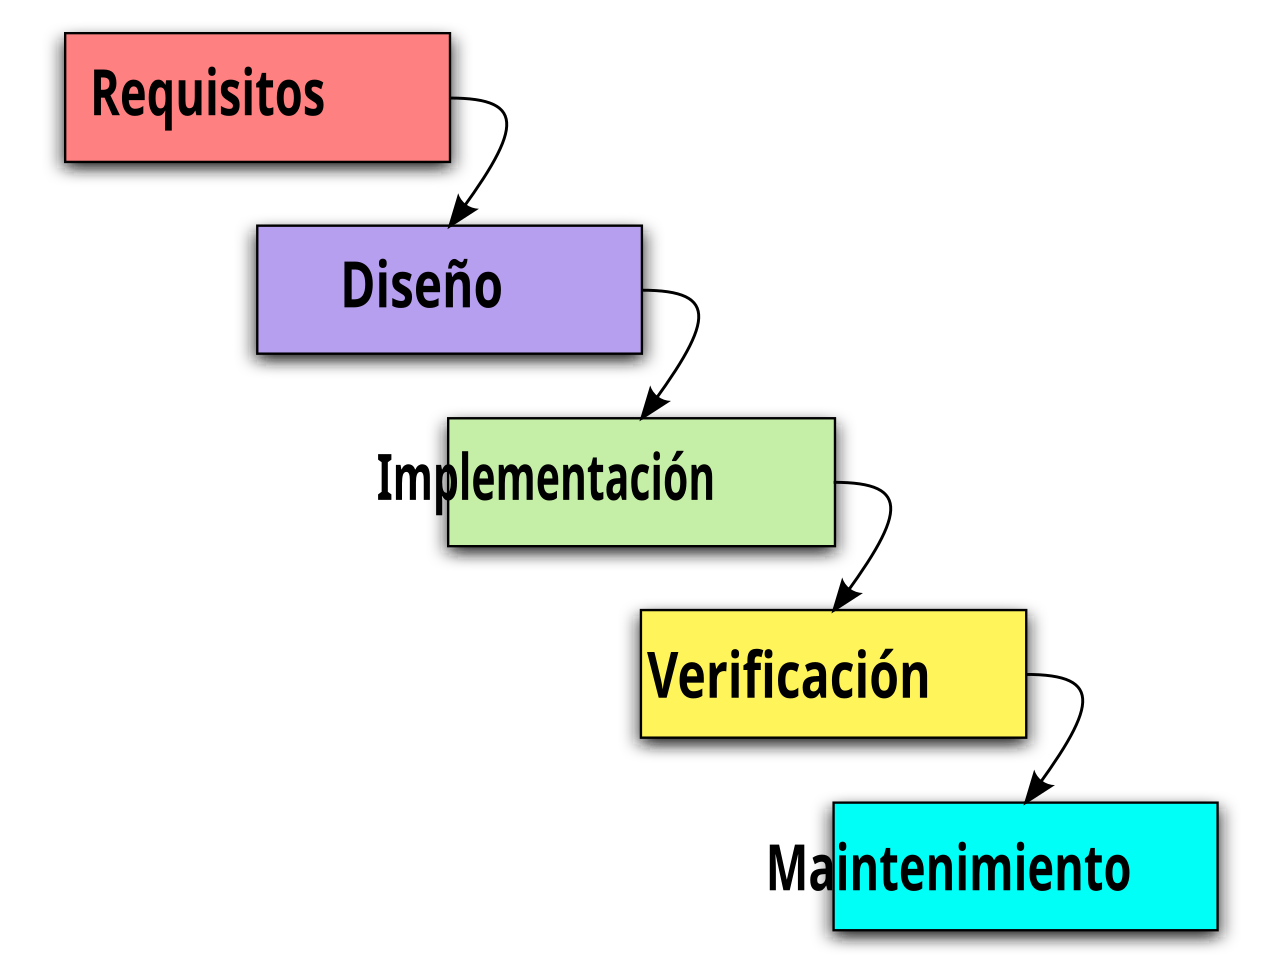
\includegraphics[width=0.5\textwidth]{Imatges/El_modelo_de_desarrollo_en_cascada.svg.png} \label{fig:Waterfall
} \caption{La secuencia de las distintas etapas del modelo de desarrollo en cascada. - Paulsmith99} \end{figure}
    

    \include{Estructura/6-Planificació}
    \chapter{Marc}
\section{Marc de treball i conceptes previs}
    \chapter{Requisits del sistema}

Com que aquest projecte no és un desenvolupament convencional de programari, els requisits es definiran per separat per a les següents parts: Màquina-Servidor, Màquina-Client i Test de Càrrega.

\section{Requisits d'una Màquina-Servidor}

Els requisits funcionals d'una Màquina-Servidor inclouen la llista de requisits imprescindibles per garantir l'accés al servidor des del Test de Càrrega de la Màquina-Client. Aquests són els següents:

\begin{itemize}
    \item La màquina ha de tenir un maquinari mínim per poder utilitzar el sistema operatiu modern que tingui instal·lat.
    \item La Màquina ha de tenir accés a Internet. 
    \item La Màquina no pot estar sota més d'un NAT\cite{wing_network_2010}, com ara un NAT massiu.\cite{richter_multi-perspective_2016} \item La Màquina ha de tenir un tallafoc instal·lat.
    \item Els ports necessaris per a la comunicació del servidor han d'estar oberts al tallafoc.\cite{liang_evolution_2022}
    \item Els ports han d'estar redirigits al router per permetre l'accés al port de la màquina des d'Internet. 
    \item La Màquina ha de tenir instal·lat i funcionant Docker Engine.  \cite{bashari_rad_introduction_2017}
\end{itemize}

Els requisits no funcionals d'una Màquina-Servidor inclouen aquells que milloren la qualitat de la prova, però no són estrictament necessaris:

\begin{itemize} 
    \item La Màquina ha de tenir components equilibrats per evitar qualsevol coll d'ampolla que pugui limitar el rendiment. \cite{singh_bottleneck_2012}
    \item La Màquina ha de tenir una connexió a Internet suficientment bona per gestionar el trànsit de dades. 
\end{itemize}

En aquest projecte, els requisits no funcionals es veuen limitats per les màquines utilitzades per a l'estudi. Per tant, aquests requisits no funcionals il·lustren les qualitats ideals d'una Màquina-Servidor, com ara una potència equilibrada i una bona connexió de xarxa.

\section{Requisits d'una Màquina-Client}

Els requisits funcionals d'una Màquina-Client inclouen els requisits imprescindibles per executar el Test de Càrrega i enviar paquets a les Màquines-Servidors. Aquests són els següents:

\begin{itemize}
    \item La Màquina ha de tenir accés a Internet. 
    \item La Màquina ha de tenir instal·lada l'eina \textit{k6}.
\end{itemize}

Els requisits no funcionals d'una Màquina-Client inclouen aquells que milloren la qualitat de la prova, però no són estrictament necessaris:

\begin{itemize} 
    \item La Màquina ha de tenir components equilibrats per evitar qualsevol coll d'ampolla que pugui limitar el rendiment. 
    \item La Màquina ha de tenir una CPU suficient per crear els \textit{Usuaris Virtuals} necessaris per a la paral·lelització de la càrrega. 
    \item La Màquina ha de tenir una connexió a Internet suficientment bona per gestionar les peticions enviades i rebudes. 
\end{itemize}

En aquest cas, és essencial que es compleixin els requisits no funcionals, ja que qualsevol limitació de la Màquina-Client podria afectar la qualitat de les dades obtingudes del rendiment dels servidors.

\section{Requisits d'un Test de Càrrega}

Els requisits funcionals d'un Test de Càrrega inclouen els requisits imprescindibles per permetre una anàlisi adequada d'un servidor HTTPS a Internet:

\begin{itemize} 
    \item El Test ha de contenir instruccions per enviar paquets al port HTTPS d'una màquina a Internet.
    \item El Test ha de retornar informació sobre les peticions fetes al servidor.
\end{itemize}

Els requisits no funcionals d'un Test de Càrrega inclouen aquells que milloren la qualitat de la prova, però no són estrictament necessaris:

\begin{itemize} 
    \item El Test ha de realitzar peticions que generin una càrrega de treball considerable. 
    \item El test ha de contenir tant contingut que no modifiqui l'estat del servidor, com contingut que sí que ho faci.
\end{itemize}
    \chapter{Estudis i decisions}
\label{cap:9}

Aquest apartat és en el qual s'expliquen les diverses eines estudiades, i el per què han estat escollides.

\section{Servidor}

Al moment de buscar servidors als que fos possible aplicar-hi una càrrega considerable, es van descartar molts en veure que la instal·lació estava trencada o que no funcionarien bé a l'hora d'estressar-los:
\subsection{Servidors no adequats per a la tasca}

\subsubsection{Colonization-Conquerors}

Tot i que aquest joc és molt ric en quant a contingut, és dependent d'una interfície d'usuari per a ser utilitzat. A més, la instal·lació i el testeig són força més complicats en ser dependent de l'editor de \textit{Godot}, un motor de videojocs. Per aquest motiu, es va optar per buscar jocs més senzills que es poguessin utilitzar des de la web.\cite{enders_timdenderscolonization-conquerors_2024}

\subsubsection{Pizza Tribes}

\textit{Pizza Tribes} és un projecte nascut a la \textit{RedisConf 2021 Hackathon}, que es va seguir desenvolupant públicament a \textit{GitHub} fins al 2023. És un projecte web amb una instal·lació més fàcil mitjançant \textit{Docker}, però és força complex en treballar amb \textit{WebSocket}, un protocol especialitzat en transferir dades en temps real a través d'internet \cite{wang_websocket_2013}. A més, el projecte no està acabat, sinó que s'ha continuat desenvolupant en privat. Per aquest motiu, es va decidir buscar un producte finalitzat, ja que així s'evitarien possibles errors en l'última versió del programari publicat, cosa que sol passar amb aquest tipus de projectes.\cite{noauthor_fnattepizza-tribes_nodate}

\subsubsection{Travian}

El joc \textit{Travian} és un RPG multijugador basat en web molt popular a internet, i el projecte en qüestió és un clon d'aquest. Tot i que ja es tenia experiència prèvia jugant a aquest joc en el passat, la instal·lació del clon és molt complicada, ja que està distribuïda en moltes pàgines, i el joc està inacabat i conté errors. Per tant, es va decidir buscar altres opcions.\cite{mousset_pierre-alexandre35travian_2024}

\subsubsection{RESTful-API-Game}


Aquest últim va cridar l'atenció, ja que utilitzava protocols generals com REST-API, un protocol utilitzat a internet per a obtenir i enviar informació de manera estandarditzada i molt simple\cite{rodriguez_rest_2016}, tot i que avui en dia és molt popular l'ús de galetes en conjunt amb REST-API, les quals permeten tenir en compte els missatges anteriors enviats al servidor, l'ús d'un backend que interaccioni mitjançant REST-API és ideal per a aquest projecte, ja que hi ha una gran quantitat d'eines disponibles per a estressar un backend amb aquest protocol\cite{li_design_2011}.

\subsection{make-apis-fun}

Finalment, buscant específicament jocs senzills que utilitzessin REST-API com a protocol d'interacció amb el backend, es va acabar trobant el backend escollit: \textit{make-apis-fun} \cite{noauthor_make-apis-funmake-apis-fun_2024}.Aquest Backend disposa de moltes virtuts per a aquest projecte:

\begin{itemize}
    \item  La primera és la facilitat d'instalació, és un servidor contenidoritzat, i tal com s'ha explicat a la \autoref{Docker}, la instanciació és a tots els sistemes operatius on estigui disponible el Docker Engine.
    \item L'altra virtud és la senzilleza de les crides gracies a ser una REST-API de caràcter purista, es a dir, que no utilitza galetes ni autentificacions i per tant és una API sense estats
    \item La tercera virtud és la seva llicencia \textit{GNU General Public License v3.0} la cual ens permet modificar-la i utilitzarla al nostre treball gracies a ser una llicencia de codi obert.
\end{itemize}

Aquests fets acabaràn sient essencials per a desenvolupar el treball, ja que aquest servidor té una gran desventatge: L'abandonament de la documentació del joc.

Aquest projecte de la cual l'ultima actualització va ser fa tres anys, encara té les instruccions generals del joc, i com instalar-lo\cite{noauthor_make-apis-fungamesclue-apireadmemd_nodate}, pero la documentació técnica de com jugar-hi s'ha perdut.L'ultim rastre que es té de la documentació dels punts d'accés està a la \textit{Wayback Machine}, una pagina que permet guardar pagines per a tal de que si en el futur desapareixesin, encara estiguin disponibles a internet en forma de copies \cite{noauthor_make_2022}. Per desgracia, l'ultima copia de 2022 no disposa de la subpagines amb la informació dels punts d'accés o com jugar-hi.Per fortuna tot i que el codi està escrit en el framework \textit{Ruby on Rails}, un llenguatge i framework que mai s'havia utilitzat, eventualment s'ha pogut deduir la manera d'interactuar amb el servidor mitjançant la lectura del codi.

Com a tallafoc per a les dues Màquines-Servidor s'ha escollit \textit{ufw}, que és un dels més populars i molt simple, adient per a sistemes simples com als nostres, i és necesari per permetre l'accés als ports desde la xarxa.\cite{noauthor_uncomplicated_nodate}

\section{Client}

Quan va quedar clar que s'utilitzaria una REST API per a comunicar-se amb el servidor, es van començar a buscar eines que permetessin fer tests de càrrega. Però abans de poder provar aquestes eines, calia esbrinar, mitjançant prova i error, com funcionava el servidor. Per fer això, inicialment es va voler utilitzar \textit{Postman}, un programa que permet enviar missatges de tipus HTTP o HTTPS en format REST API, que habitualment s'utilitza per verificar que els punts d'accés d'un servidor responen amb el contingut correcte. A causa de les dificultats causades per la monetització de Postman, i per afinitat amb programes de codi obert, es va canviar Postman per \textit{Hoppscotch}, que, essencialment, compleix les mateixes funcions.\cite{noauthor_hoppscotch_nodate}

Un cop descoberts alguns punts d'accés bàsics, es va fer la selecció entre les diverses eines disponibles per a generar tests de càrrega. La primera eina que es va estudiar va ser \textit{Apache JMeter}. Aquesta permet fer moltes crides, però les guies d'instal·lació i execució la mostraven com bastant complicada \cite{noauthor_how_nodate}. En canvi, l'eina k6, escrita en Go i de codi obert, s'utilitza com a llibreria de JavaScript ES6 \cite{simpson_you_2015}, i resulta en un codi molt senzill que es pot executar fàcilment sense necessitat d'interfície gràfica.\cite{noauthor_running_nodate}
    \include{Estructura/10-Anàlisi}
    \include{Estructura/11-ImplementacióProves}
    \include{Estructura/12-ImplementacióResultats}
    \chapter{Conclusions}
\section{Conclusions}
    \chapter{Treball futur}

Expansions d'aquest estudi i treball es poden centrar en els següents apartats: \begin{itemize} 
\item Realitzar més proves amb aquestes dues màquines. 
\item Repetir els experiments, però amb la màquina local connectada per cable \textit{Ethernet} en comptes de \textit{Wi-Fi}. 
\item Canviar la màquina al núvol per una altra amb més capacitat de processament i memòria. 
\item Experimentar amb altres programes que facin de servidor d'un joc senzill. 
\item Utilitzar altres eines per a fer tests de càrrega i comparar el seu rendiment amb \textit{k6}. 
\item Adaptar el joc senzill actual perquè pugui ser utilitzat com a \textit{AWS Lambda}, \textit{Google Cloud Functions} o \textit{Azure Functions} al núvol, una arquitectura alternativa a una màquina virtual on, en comptes de cobrar pel temps que la màquina està encesa, es cobra per la quantitat de peticions realitzades. 
\item Fer que més d'una Màquina actuï com a client simultàniament per aproximar-se millor a una càrrega distribuïda real. 
\item Traslladar la Màquina-Servidor local a una xarxa d'una altra companyia de telecomunicacions ubicada a la mateixa ciutat, per observar si hi ha variabilitat en la connexió entre la Màquina-Client i la Màquina-Servidor local. 
\item Experimentar amb diferents patrons de càrrega en lloc d'utilitzar increments lineals.
\end{itemize}
    \chapter{Bibliografia}

\printbibliography[title={}, heading=none, notkeyword={Annexos}]

    \chapter{Annexos}

\printbibliography[title={}, heading=none, keyword={Annexos}]

    \chapter{Manual}
\section{Manual d'usuari i/o instalació}
    
    
  

    %Bibliografia
    \addcontentsline{toc}{part}{Bibliografia}
    \bibliographystyle{plainnat}
    \bibliography{referències}

\end{document}
